\section{Literature Review}
\label{sec:review}

\subsection{Maintenance Strategies and Predictive Maintenance}
\label{sec:pdm}

The railway survey by \citet{davari2021survey} distinguishes three generations of maintenance. \emph{Corrective} or run-to-failure maintenance repairs equipment after it has failed; \emph{preventive} maintenance performs scheduled tasks to reduce the probability of failure; and \emph{predictive} maintenance requires direct monitoring of the mechanical condition so that interventions can be planned when degradation is actually observed. \citet{silva2023adversarial} summarise the economic trade-off behind this sequence: preventive maintenance may replace components that are still healthy, whereas corrective maintenance causes losses through vehicle or production shutdowns. PdM is attractive precisely because it promises to avoid both.

Within PdM, two perspectives are common \citep{davari2021survey}. \emph{Failure prediction} asks whether, and when, a failure will occur within a horizon, while \emph{remaining useful life} (RUL) estimation predicts the time left until the end of a component's life. Prognostic approaches can further be classified as model-based, knowledge-based or data-driven \citep{davari2021survey}. Model-based and knowledge-based approaches require physical models or expert rules of the degradation process; data-driven approaches learn the relevant patterns from monitoring data and are the focus of recent work on railway vehicles.

The same survey identifies the obstacles that are characteristic of railway PdM \citep{davari2021survey}. Labelling continuous sensor streams is expensive, so ``using supervised learning is not a feasible solution'' in this context; the high volume of time series has to be processed in (near) real time; commonly used evaluation metrics do not fit the operational setting; and maintenance decisions require some form of causal explanation, for instance by linking machine-learning results to root-cause analysis. As a consequence, the survey frames railway PdM as a problem of \emph{anomaly detection on time series} and recommends recurrent neural networks, generative models, transfer learning and reinforcement learning as directions for future work.

For our case study these observations translate into three requirements. First, with four documented failures, RUL estimation is not feasible and the task is formulated as early failure warning. Second, the detector must learn from data assumed to be normal, i.e.\ it is unsupervised or semi-supervised. Third, evaluation and explanation must be designed with the operator in mind. The following subsections review the literature that addresses these three requirements.

\subsection{Anomaly Detection in Multivariate Time Series}
\label{sec:ad}

\paragraph{Definitions and taxonomy.}
\citet{ruff2021unifying} define an anomaly as ``an observation that deviates considerably from some concept of normality'' and treat the terms anomaly, outlier and novelty interchangeably. Formally, anomalies lie in low-probability regions of the distribution of normal data, and most detectors explicitly or implicitly estimate these low-density regions. For time series, \citet{blazquez2021review} propose a taxonomy along three axes: the input data (univariate or multivariate), the type of outlier (a single \emph{point}, a \emph{subsequence} of consecutive points whose joint behaviour is unusual, or a whole time series that differs from the others) and the nature of the detection method (analysing each variable separately or several variables jointly). In this taxonomy, an air leak in the APU is best understood as a \emph{multivariate subsequence anomaly}: no single reading is necessarily abnormal, but the joint behaviour of pressures, motor current and duty cycle over minutes to hours differs from normal operation.

\paragraph{Method families.}
\citet{ruff2021unifying} unify detectors into three families. \emph{Probabilistic} models estimate the density of normal data; \emph{one-class classification} methods learn a boundary around normal data without estimating the full density; and \emph{reconstruction} models, from principal component analysis (PCA) to autoencoders, learn to reproduce normal data and use the reconstruction error as anomaly score. The authors argue that the core principle is the same for ``shallow'' methods with a fixed feature representation and ``deep'' methods that learn the representation, but deep methods introduce more hyper-parameters and usually require more data. They also name the mostly unsupervised nature of the problem, contamination of training data with anomalies, limited interpretability and non-stationarity of the data as central challenges.

Two shallow and two deep approaches are particularly relevant for our project. \emph{Isolation Forest} \citep{liu2008isolation} departs from profiling normal behaviour and instead isolates anomalies explicitly with random partitions; it uses sub-sampling, has linear time complexity and low memory requirements, handles high-dimensional data and, according to its authors, also works when the training set contains no anomalies. \emph{Autoencoders} learn a compressed, nonlinear representation of normal data; \citet{sakurada2014autoencoders} report on spacecraft telemetry that autoencoders detect subtle anomalies that linear PCA misses. For sequential data, autoencoders are built from recurrent units, most commonly long short-term memory (LSTM) cells \citep{hochreiter1997lstm}. \citet{malhotra2016lstm} train an LSTM encoder--decoder only on normal sequences and score each time step by the likelihood of its reconstruction error under a Gaussian fitted on validation data; their approach also detects anomalies in series that are hard to predict, where prediction-based detectors struggle. As an alternative, \citet{hundman2018detecting} predict each telemetry channel with an LSTM and flag anomalies when smoothed prediction errors exceed a non-parametric, dynamically chosen threshold.

\paragraph{Evidence from benchmarks.}
Whether deep detectors are worth their cost is an empirical question. In the largest comparative evaluation we found, \citet{schmidl2022anomaly} collected and re-implemented 71 algorithms and evaluated them on 976 time series. They conclude that there is ``no clear winner'', that simple methods perform almost as well as sophisticated ones, and that deep-learning approaches are ``not (yet) competitive'' given their training effort; many reconstruction-based methods reached an AUC-ROC of only about 0.5. They also show that rankings change with the evaluation metric. For a small, safety-relevant application this is a strong argument to benchmark deep models against simple baselines rather than against each other only.

\paragraph{From scores to alarms.}
All detectors above produce a continuous score that must be converted into alarms. Proposed rules range from thresholds optimised on labelled validation data \citep{malhotra2016lstm} over statistics of the training errors, such as $Q_3 + 3\,\mathrm{IQR}$ \citep{silva2023adversarial,gama2024neurosymbolic}, to the non-parametric threshold of \citet{hundman2018detecting}. Because isolated high scores are frequent in noisy sensor data, a second stage is often added. \citet{ribeiro2016sequential} pass the binary output of a point detector through a low-pass filter $y_i = y_{i-1} + \alpha (x_i - y_{i-1})$ and raise an alarm only when the filtered signal exceeds 0.5, so that only \emph{sequences} of anomalies trigger an alarm; this ``strong impact in the false alarm rate'' was their main result. \citet{hundman2018detecting} prune anomalous sequences whose scores are not clearly separated from normal noise, which raised precision from 48.9\,\% to 87.5\,\% at a small loss of recall. They also stress the operational side: ``investigation of even a couple false positives can deter users''.

\paragraph{Non-stationarity.}
Detectors trained on one period assume that normal behaviour remains stable. \citet{ruff2021unifying} list distribution shift as an open challenge, and the concept-drift literature studies how models can adapt when the data-generating process changes over time \citep{gama2014drift}. The latter is formulated mainly for supervised learning, but the underlying issue --- that normal behaviour in the training period may not represent later periods --- also affects unsupervised detectors trained on a single month of data, as in our case (Section~\ref{sec:outline}).

\subsection{Evaluating Anomaly Detectors for Maintenance}
\label{sec:eval}

Classical precision and recall treat every time step independently. \citet{tatbul2018precision} point out that many real-world anomalies are \emph{range-based}, i.e.\ they last over a period of time, and extend precision and recall to ranges with options for domain-specific preferences. A widespread shortcut in the literature is \emph{point adjustment} (PA): if any point of an anomalous segment is detected, the whole segment is counted as detected. \citet{kim2022rigorous} show that PA can grossly overestimate performance; on the SWaT benchmark even a \emph{random} anomaly score reached an F1 of 0.969 after PA, compared with 0.216 without it. They propose PA\%K, which applies PA only if at least $K$\,\% of a segment is detected, and recommend comparing new methods against an untrained model as a baseline.

\citet{wu2021flawed} question benchmark datasets themselves and identify four recurring flaws: \emph{triviality} (problems solvable with one line of code), \emph{unrealistic anomaly density}, \emph{mislabelled ground truth} and \emph{run-to-failure bias} (anomalies concentrated at the end of a series). Two of these are directly relevant to MetroPT-3: ground truth comes from maintenance reports whose start and end times are approximate, and with only four events, a single mislabelled event changes recall by 25 percentage points.

For PdM, the \emph{timing} of a detection matters as much as its existence. The Numenta Anomaly Benchmark \citep{lavin2015nab} defines a window around each labelled anomaly, gives credit only to the earliest detection inside the window, rewards earlier detections more through a scaled sigmoid and penalises detections outside windows as false positives; application profiles weight false positives or false negatives more strongly. The Metro do Porto use case defines its own operational protocol: a predicted failure interval is a true positive if it overlaps a reported failure, a predicted interval without overlap is a false positive and a missed failure is a false negative \citep{veloso2022metropt}. A detection counts as \emph{early} if it occurs at least two hours before the train becomes non-operational \citep{veloso2022metropt}, operationalised by \citet{silva2023adversarial} as two hours before the low-pressure signal (LPS), a digital alarm that becomes active when the system pressure falls below 7\,bar. Warnings closer than 24 hours are merged into one \citep{silva2023adversarial}.

Taken together, this literature suggests evaluating at the level of \emph{events} rather than time steps, avoiding point adjustment, reporting lead time and false alarms explicitly and, given the very small number of failures, reporting results per event rather than as a single aggregated score.

\subsection{Explainable AI for Maintenance Decisions}
\label{sec:xai}

\citet{vollert2021interpretable} observe that many PdM studies rely on non-interpretable models and that a lack of explainability may lead to a lack of trust. Among the challenges they identify are the evaluation of interpretability, explanation methods that are themselves black boxes, inconsistent terminology and limited work on time-series data. The survey by \citet{cummins2024xpdm}, which screened 6{,}932 records and included 102 articles, distinguishes post-hoc \emph{explainable AI} (XAI), which explains an already trained model, from \emph{interpretable machine learning} (iML), which uses models that are understandable by design, and \emph{local} explanations of single predictions from \emph{global} explanations of the whole model. Anomaly detection is the most common PdM task in which these techniques are applied, and SHAP is ``by far'' the most used method, followed by LIME. The survey also reports studies in which SHAP and LIME produced diverging explanations for the same model.

LIME \citep{ribeiro2016lime} explains a single prediction of any classifier by fitting an interpretable model locally around that prediction. SHAP \citep{lundberg2017shap} frames feature attribution as an additive explanation model and shows that Shapley values from cooperative game theory are the unique additive attribution that satisfies three properties: \emph{local accuracy} (the attributions sum to the model output), \emph{missingness} and \emph{consistency}. Model-agnostic (Kernel SHAP) and model-specific approximations (e.g.\ Deep SHAP for neural networks) make the method applicable to the detectors discussed above.

In the Metro do Porto studies, two explanation styles coexist. One line of work trains an online rule learner (AMRules) to predict the anomaly score from the sensor values and presents the rules that cover an alarm \citep{silva2023adversarial,gama2024neurosymbolic}. Its authors argue that rules can be generated in real time and are easier to read because they contain only a few conditions, whereas SHAP lists the contribution of every feature; in one case the rules pointed to the sensor that maintenance later identified as the root cause \citep{silva2023adversarial}. The other line applies SHAP to the detector \citep{davari2024explaining}. \citet{garciamendez2025explainable} go further and generate natural-language and visual explanations in an online pipeline. In the studies whose full text we could read, explanation quality is assessed qualitatively, for example through feedback from maintenance engineers \citep{gama2024neurosymbolic} or by relating rules to the root cause recorded in maintenance reports \citep{silva2023adversarial}.

\subsection{Railway Predictive Maintenance}
\label{sec:railway}

The survey by \citet{davari2021survey} covers infrastructure (tracks, switches), maintenance scheduling and rolling stock, including wheels, bearings, traction, doors, and air compressors and brake pipes. It notes that railway-specific literature is still scarce and that few studies treat the sensor data explicitly as time series. The most detailed body of work on a single railway component that we found concerns the APU of Metro do Porto trains; it is reviewed study by study in the next section.

\section{Studies on the Metro do Porto Air Production Unit}
\label{sec:metropt}

This section summarises, in chronological order, the studies most closely related to our project. Almost all of them originate from the research group at INESC TEC and the University of Porto that published the MetroPT datasets. For each study we state its key insight and its relevance for our case study. Where only the abstract was available, this is indicated.

\subsection[Ribeiro et al. (2016): Sequential Anomalies in the Railway Industry]{Sequential Anomalies: A Study in the Railway Industry}
\textbf{Authors:} R.~P.~Ribeiro, P.~Pereira, J.~Gama (2016), \textit{Machine Learning} \cite{ribeiro2016sequential}\\
This study predicts failures of automatic train doors from sensor data of the pneumatic valves that open and close them. A single abnormal door cycle is usually caused by passengers, not by the equipment, so the goal is to detect \emph{sequences} of abnormal cycles. The authors compare outlier, anomaly and novelty detectors and propose a two-stage architecture in which the binary output of a point detector is smoothed by a low-pass filter $y_i = y_{i-1} + \alpha (x_i - y_{i-1})$; an alarm is raised when the filtered signal exceeds 0.5.\\
\textbf{Key Insight:} The low-pass filter had a ``strong impact in the false alarm rate''.\\
\textbf{Relevance:} Our threshold baseline raises many short false-alarm episodes; the same post-processing is planned for all our detectors.

\subsection[Barros (2020): APU in EuroTram Vehicles]{Predictive Maintenance for Air Production Unit in EuroTram Vehicles}
\textbf{Author:} M.~C.~de~Barros (2020), Master's thesis, University of Porto \cite{barros2020thesis}\\
Within the FailStopper project of Metro do Porto and INESC TEC, the thesis analyses two APUs between March and July 2020, which overlaps the MetroPT-3 period. Data were acquired at 1\,Hz, and one unit lists four air leaks of the pneumatic panel. The author tests six rules based on the frequency and duration of signal peaks, clustering (K-Means, DBSCAN) and autoencoders. The best single rule predicted 87.5\,\% of the reported failures with a reported false-alarm rate of 37\,\%; DBSCAN predicted half of the failures at least one hour in advance, a simple autoencoder only five minutes in advance. The thesis also reports a missing flow meter and an oil-level sensor installed in reverse on one unit.\\
\textbf{Key Insight:} Simple rules already detect most failures on the 2020 data, but at the cost of many false alarms.\\
\textbf{Relevance:} The only openly available analysis of the 2020 APU data; a reference point for our threshold baseline and a source for the failure dates (it lists the fourth air leak on 17 July, the UCI page on 15 July).

\subsection[Davari et al. (2021): Deep Anomaly Detection for the APU]{Predictive Maintenance Based on Anomaly Detection Using Deep Learning for Air Production Unit in the Railway Industry}
\textbf{Authors:} N.~Davari, B.~Veloso, R.~P.~Ribeiro, P.~M.~Pereira, J.~Gama (2021), \textit{IEEE DSAA} \cite{davari2021dsaa} --- abstract only\\
According to the abstract, a sparse autoencoder detects abnormal sensor data of the APU, with separate variants for analogue and digital sensors. Air leaks were best detected from analogue data, alarms were triggered by a low-pass filter and a sequence of abnormal readings, and the sparse autoencoder outperformed a variational autoencoder in precision, recall and F1. In the same year, the same authors published the MetroPT-3 dataset \cite{davari2021metropt3data}.\\
\textbf{Key Insight:} Reconstruction-based deep detection combined with alarm smoothing is feasible on the APU data.\\
\textbf{Relevance:} The first deep-learning baseline associated with the 2020 data.

\subsection[Veloso et al. (2022): The MetroPT Dataset]{The MetroPT Dataset for Predictive Maintenance}
\textbf{Authors:} B.~Veloso, R.~P.~Ribeiro, J.~Gama, P.~M.~Pereira (2022), \textit{Scientific Data} \cite{veloso2022metropt}\\
The paper describes a second data collection, MetroPT, recorded from January to June 2022 at 1\,Hz with eight analogue, eight digital and four GPS signals and three reported failures (two air leaks, one oil leak). It explains the role of the APU, states the operator's requirement of detection at least two hours before the train becomes non-operational, defines interval-overlap rules for true and false positives, and notes that APU failures are typically undetectable with threshold-based condition monitoring. According to the authors, the data contain no missing values.\\
\textbf{Key Insight:} Defines the operational goals and evaluation logic of the Metro do Porto use case.\\
\textbf{Relevance:} Basis for our event-level evaluation; the contrast with the gaps in MetroPT-3 motivates our data-quality analysis.

\subsection[Meira et al. (2023): Data-Driven PdM Framework]{Data-Driven Predictive Maintenance Framework for Railway Systems}
\textbf{Authors:} J.~Meira, B.~Veloso, V.~Bol\'on-Canedo, G.~Marreiros, A.~Alonso-Betanzos, J.~Gama (2023), \textit{Intelligent Data Analysis} \cite{meira2023framework} --- abstract only\\
According to the abstract, the framework combines Half-Space-Trees with a one-class $k$-nearest-neighbour detector adapted to streaming data from the APU. Compared with Half-Space-Trees alone, the combination produces fewer type-I errors and higher precision, and it predicts most of the catastrophic failures. The abstract does not state which data version was used.\\
\textbf{Key Insight:} Shallow, streaming detectors can be competitive on the APU data.\\
\textbf{Relevance:} Supports including a shallow detector (Isolation Forest) in our comparison.

\subsection[Silva et al. (2023): Adversarial Autoencoders and Explainability]{Predictive Maintenance, Adversarial Autoencoders and Explainability}
\textbf{Authors:} M.~E.~P.~Silva, B.~Veloso, J.~Gama (2023), \textit{ECML PKDD} \cite{silva2023adversarial}\\
Using three months of the 2022 data, the authors train on the first month (assumed normal) and test on the following two. They compare LSTM, temporal-convolutional and Wasserstein adversarial autoencoders on compressor cycles and on 30-minute windows, set the threshold at $Q_3 + 3\,\mathrm{IQR}$ of the training errors, smooth alarms with a low-pass filter, merge warnings closer than 24 hours and count a detection as early if it occurs at least two hours before the low-pressure signal (LPS). On windows, the adversarial model detected both failures early without false alarms; the LSTM autoencoder avoided false alarms but did not detect the air leak early. Alarms are explained with AMRules, an online rule learner, which the authors consider more suitable for real-time use than LIME or SHAP.\\
\textbf{Key Insight:} Window-based input and adversarial training gave early, false-alarm-free detection on two failures.\\
\textbf{Relevance:} Same training protocol as ours and a concrete operational definition of ``early''.

\subsection[Gama et al. (2024): Neuro-Symbolic Explainer for Rare Events]{A Neuro-Symbolic Explainer for Rare Events}
\textbf{Authors:} J.~Gama, R.~P.~Ribeiro, S.~Mastelini, N.~Davari, B.~Veloso (2024), arXiv preprint \cite{gama2024neurosymbolic}\\
An LSTM autoencoder on compressor cycles of the 2022 data flags anomalies with a $Q_3 + 3\,\mathrm{IQR}$ threshold and a low-pass filter. In parallel, AMRules learns to predict the reconstruction error from the sensor values, which yields global rules (for engineers) and local rules for single alarms (for the workshop); an over-sampling step based on Chebyshev's inequality emphasises rare events. The rules are compared with SHAP and found easier to read, and, according to the authors, the maintenance team found that the model helped them understand APU behaviour not described by the manufacturer.\\
\textbf{Key Insight:} Rule-based explanations can be produced online alongside a deep detector.\\
\textbf{Relevance:} An alternative to SHAP against which our explanations can be compared qualitatively.

\subsection[Davari et al. (2024): Detecting and Explaining APU Anomalies]{Detecting and Explaining Anomalies in the Air Production Unit of a Train}
\textbf{Authors:} N.~Davari, B.~Veloso, R.~P.~Ribeiro, J.~Gama (2024), \textit{ACM SAC} \cite{davari2024explaining} --- abstract only\\
According to the abstract, the study uses MetroPT-3 and proposes an LSTM autoencoder framework that identifies abnormal data and reduces false alarms. It outperforms the earlier sparse autoencoder in F1, recall and precision and uses SHAP to show which features drive the detections.\\
\textbf{Key Insight:} LSTM autoencoder with SHAP is already established on MetroPT-3.\\
\textbf{Relevance:} The closest prior work; our project must position itself against it (Section~\ref{sec:map}).

\subsection[Jakobs et al. (2025): Interpretable Rules for Online Failure Prediction]{Interpretable Rules for Online Failure Prediction}
\textbf{Authors:} M.~Jakobs, B.~Veloso, J.~Gama (2025), arXiv preprint \cite{jakobs2025rules}\\
On the MetroPT2 data (April--July 2022), a convolutional autoencoder on 30-minute windows produces a failure probability, and an online rule learner explains it. The approach reached a perfect F1 score on the two failures of the test period, detecting the air leak more than 150 minutes before the LPS signal. The best rules depend on a flow-meter sensor that is expensive and not available on all trains. The authors report that they ``struggled to fit a good Autoencoder onto MetroPT3'' and recommend that future work ``should also focus on MetroPT3''.\\
\textbf{Key Insight:} Results on the 2022 data partly rely on a sensor that MetroPT-3 does not contain.\\
\textbf{Relevance:} Explicit recommendation to study MetroPT-3 as the more challenging dataset.

\subsection[Garc\'ia-M\'endez et al. (2025): Explainable ML Framework for Railway PdM]{An Explainable Machine Learning Framework for Railway Predictive Maintenance}
\textbf{Authors:} S.~Garc\'ia-M\'endez, F.~de~Arriba-P\'erez, F.~Leal, B.~Veloso, B.~Malheiro, J.~C.~Burguillo-Rial (2025), arXiv preprint \cite{garciamendez2025explainable}\\
The authors label the two hours before each reported failure in the 2022 data as positive and train incremental classifiers on statistical and frequency features with prequential evaluation (predict, then update). Explanations are generated in natural language and as visualisations. They report an F-measure above 98\,\%.\\
\textbf{Key Insight:} A supervised, streaming formulation with user-oriented explanations.\\
\textbf{Relevance:} Shows a different problem formulation; with four events and an unsupervised setting, we do not follow it.

\section{Literature Map and Research Gap}
\label{sec:map}

\subsection{Summary of Reviewed Works}
Figure~\ref{fig:map} summarises how the reviewed themes build on each other and feed into our project, and Table~\ref{tab:apu} compares the studies on the Metro do Porto APU.

\begin{figure}[!tb]
\centering
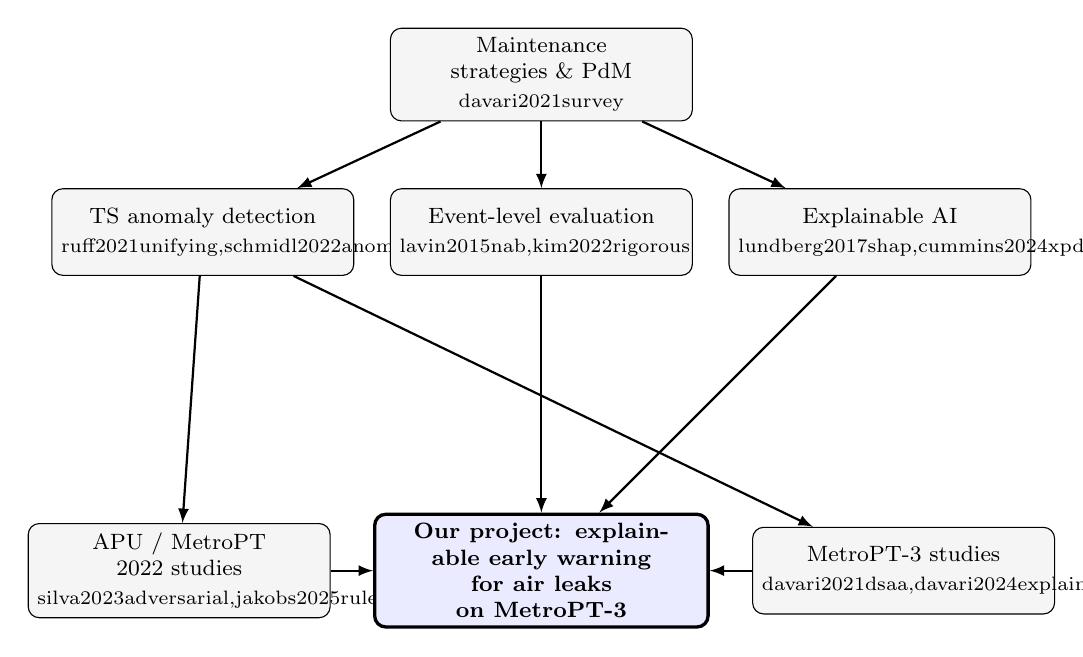
\begin{tikzpicture}[
  box/.style={draw, rounded corners, align=center, font=\footnotesize, minimum height=1.1cm, text width=3.6cm, fill=gray!8},
  core/.style={draw, very thick, rounded corners, align=center, font=\footnotesize\bfseries, text width=4.0cm, minimum height=1.2cm, fill=blue!8},
  arr/.style={-{latex}, thick}]
\node[box] (pdm) at (0,3.2) {Maintenance strategies \& PdM\\[1pt]\scriptsize \citet{davari2021survey}};
\node[box] (ad) at (-4.3,1.2) {TS anomaly detection\\[1pt]\scriptsize \citet{ruff2021unifying,schmidl2022anomaly}};
\node[box] (ev) at (0,1.2) {Event-level evaluation\\[1pt]\scriptsize \citet{lavin2015nab,kim2022rigorous}};
\node[box] (xai) at (4.3,1.2) {Explainable AI\\[1pt]\scriptsize \citet{lundberg2017shap,cummins2024xpdm}};
\node[box] (apu) at (-4.6,-3.1) {APU / MetroPT 2022 studies\\[1pt]\scriptsize \citet{silva2023adversarial,jakobs2025rules}};
\node[box] (m3) at (4.6,-3.1) {MetroPT-3 studies\\[1pt]\scriptsize \citet{davari2021dsaa,davari2024explaining}};
\node[core] (us) at (0,-3.1) {Our project: explainable early warning\\ for air leaks on MetroPT-3};
\draw[arr] (pdm) -- (ad); \draw[arr] (pdm) -- (ev); \draw[arr] (pdm) -- (xai);
\draw[arr] (ad) -- (apu); \draw[arr] (ad) -- (m3);
\draw[arr] (ev) -- (us); \draw[arr] (xai) -- (us);
\draw[arr] (apu) -- (us); \draw[arr] (m3) -- (us);
\end{tikzpicture}
\caption{Literature map: from general themes (top) to the specific APU studies and our project (bottom).}
\label{fig:map}
\end{figure}

\begin{table}[H]
\centering
\caption[Studies on the Air Production Unit of Metro do Porto trains]{Studies on the Air Production Unit of Metro do Porto trains. FA = false alarms; AE = autoencoder; ``abstract'' = only the abstract was available to us.}
\label{tab:apu}
\footnotesize
\setlength{\tabcolsep}{3pt}
\begin{tabular}{>{\raggedright\arraybackslash}p{2.4cm}>{\raggedright\arraybackslash}p{1.8cm}>{\raggedright\arraybackslash}p{3.3cm}>{\raggedright\arraybackslash}p{1.9cm}>{\raggedright\arraybackslash}p{4.4cm}}
\toprule
Study & Data & Detector & Explanation & Reported result (early warning / FA) \\
\midrule
\citet{barros2020thesis} & APU 2020 & Peak rules, DBSCAN, AE & -- & Best rule: 87.5\,\% of failures, 37\,\% FA; DBSCAN 50\,\% $\geq$1\,h ahead \\
\citet{davari2021dsaa} & APU (abstract) & Sparse AE + low-pass filter & -- & SAE better than VAE (abstract) \\
\citet{meira2023framework} & APU (abstract) & Half-Space-Trees + 1-class $k$NN, streaming & -- & Fewer type-I errors (abstract) \\
\citet{silva2023adversarial} & MetroPT 2022 & LSTM / TCN / WAE-GAN AE & AMRules & WAE-GAN: both failures $\geq$2\,h before LPS, 0 FA \\
\citet{gama2024neurosymbolic} & MetroPT 2022 & LSTM-AE (cycles) & AMRules + SHAP comparison & All train-removal failures detected \\
\citet{davari2024explaining} & MetroPT-3 (abstract) & LSTM-AE & SHAP & Better than SAE (abstract) \\
\citet{jakobs2025rules} & MetroPT2 2022 & Conv.\ AE & Online rules & Perfect F1 on 2 failures; flow-meter dependent \\
\citet{garciamendez2025explainable} & MetroPT 2022 & Incremental classifiers (supervised) & Text + visual & F-measure $>$98\,\% \\
\bottomrule
\end{tabular}
\end{table}

\subsection{Synthesis and Observations}
Four observations follow from the map and the table.
\begin{enumerate}[label=\textbf{G\arabic*}, leftmargin=*, itemsep=3pt]
  \item \textbf{MetroPT-3 is less explored and considered harder.} Most recent studies use the 2022 data, which contain a flow meter and are reported to have no missing values. Apart from the 2020 thesis \citep{barros2020thesis}, only two studies on the 2020 data were found \citep{davari2021dsaa,davari2024explaining}, both accessible to us only as abstracts, and \citet{jakobs2025rules} explicitly recommend MetroPT-3 as a more challenging target.
  \item \textbf{Simple baselines are rarely part of the comparison.} The APU studies compare deep architectures with each other, whereas large benchmarks find simple methods to be competitive \citep{schmidl2022anomaly}. Apart from the rules in \citet{barros2020thesis} and the streaming detector of \citet{meira2023framework}, we found no APU study that compares a threshold rule or a shallow detector such as Isolation Forest with a deep model under the same protocol.
  \item \textbf{Evaluation protocols differ.} Studies use compressor cycles, fixed windows or prequential classification; early detection is defined relative to the LPS signal or the reported failure; and results rest on two to four events. Lead time and false alarms per day are not reported in a common format, and point-adjustment effects \citep{kim2022rigorous} are not discussed in the studies we could read in full.
  \item \textbf{Data quality is hardly discussed.} The dataset paper of the 2022 data reports no missing values \citep{veloso2022metropt}; for MetroPT-3, recording gaps, frozen logging periods or the difference between the 1\,Hz acquisition described by \citet{barros2020thesis} and the roughly 10-second resolution of the public file are not addressed in the sources available to us.
\end{enumerate}

\subsection{Alignment with the Proposed Work}
Table~\ref{tab:align} maps these observations to the design of our case study.

\begin{table}[H]
\centering
\caption{Alignment of the research insights with the proposed work.}
\label{tab:align}
\small
\begin{tabular}{>{\raggedright\arraybackslash}p{2.6cm}>{\raggedright\arraybackslash}p{5.6cm}>{\raggedright\arraybackslash}p{5.6cm}}
\toprule
Criterion & Research insight & Proposed work \\
\midrule
Dataset & 2022 data dominate; MetroPT-3 recommended as harder \cite{jakobs2025rules} & Full study on MetroPT-3 (2020) \\
Detectors & Simple methods often competitive \cite{schmidl2022anomaly}; APU studies compare deep models & Threshold rule, Isolation Forest and LSTM autoencoder under one protocol \\
Alarm logic & Low-pass filtering reduces false alarms \cite{ribeiro2016sequential,silva2023adversarial} & Same threshold and filter for all detectors \\
Evaluation & Point adjustment inflates scores \cite{kim2022rigorous}; early $=$ $\geq$2\,h before LPS \cite{silva2023adversarial} & Event-level recall, lead time, false alarms per day, reported per failure \\
Data quality & Not discussed for MetroPT-3 & Gaps and frozen segments detected and masked \\
Explanation & SHAP or online rules \cite{davari2024explaining,gama2024neurosymbolic} & SHAP per alarm, compared qualitatively with rule-based results \\
Reproducibility & Results rest on two to four events; protocols differ between studies & Open repository, fixed seeds, chronological split, per-failure results \\
\bottomrule
\end{tabular}
\end{table}

\paragraph{Positioning.}
Compared with the closest study \citep{davari2024explaining}, our project does not claim novelty for combining an LSTM autoencoder with SHAP on MetroPT-3. Its intended contribution lies in the gaps G2--G4: a transparent, leakage-free benchmark of a threshold rule, Isolation Forest and an LSTM autoencoder under one chronological protocol; event-level evaluation with lead time and false alarms per day, aligned with the operator's two-hour requirement; an explicit treatment of the data-quality issues of MetroPT-3; and openly available, reproducible code.

\section{Method Outline}
\label{sec:outline}

\subsection{First Findings from the Data}
A first EDA of the full MetroPT-3 file (1{,}516{,}948 records) confirmed the record count of the UCI description and found no missing values and no duplicate timestamps. Several findings, however, directly affect the method:
\begin{itemize}[itemsep=2pt]
  \item \textbf{Sampling and gaps.} The median interval between records is 10\,s, not 1\,s. There are 275 recording gaps longer than five minutes, covering 17.7\,\% of the period; 29 February 2020 is missing entirely.
  \item \textbf{Frozen logging.} Nine segments of at least 30 minutes, 7 days and 2 hours in total (3.3\,\% of records), show all analogue signals at exactly constant values. One of them covers the hours directly before failure~1 (17~April 09:20 to 18~April 00:18).
  \item \textbf{Operating states.} The motor current has three clear states (about 0\,A, 3.8\,A and 5.4--6.3\,A), which differ from the 4\,A and 7\,A levels in the dataset description.
  \item \textbf{Failure signature.} During the four failures the compressor runs under load almost continuously (mean hourly load ratio 0.975), whereas the 24 hours before a failure (0.161) are close to normal operation (0.145): leaks are easy to see once they occur, but hard to anticipate.
  \item \textbf{Distribution shift.} February, the training month, shows a lower duty cycle and oil temperature than March to August.
  \item \textbf{Label uncertainty.} The UCI page dates failure~4 on 15~July 2020, whereas the failure table in \citet{barros2020thesis} lists 17~July 2020 for the fourth air leak of the unit analysed there; whether this is the same unit cannot be confirmed from the available sources.
\end{itemize}

\subsection{Threshold Baseline}
As a first baseline we aggregated the signals into 10-minute windows and raised an alarm when at least two of four rules (low minimum TP3 and reservoir pressure, high share of time under load, high mean motor current), with thresholds at the 1\,\%/99\,\% quantiles of February, fired in three consecutive windows. On the test period (March--August) it detected all four failures, but only failure~4 before its reported start (120 minutes ahead); failures 1--3 were detected 50, 20 and 20 minutes after the reported start. It raised 45 false-alarm episodes (about 0.24 per day) with a window-level precision of 0.32 and recall of 0.91. The longest false-alarm block lies inside a frozen segment. In line with \citet{veloso2022metropt}, a simple threshold approach therefore detects ongoing leaks but provides almost no early warning.

\subsection{Planned Pipeline}
Building on the literature, the next project stages will proceed as follows.
\begin{enumerate}[itemsep=2pt]
  \item \textbf{Preprocessing.} Mask frozen segments and treat recording gaps explicitly (no windows across gaps); fit all normalisation parameters on the training period only.
  \item \textbf{Chronological split.} Train on February (normal operation, as in \citet{silva2023adversarial}); use a later failure-free period for threshold calibration; evaluate on the remaining months. The February shift is reported as a limitation.
  \item \textbf{Detectors.} Threshold baseline (done), Isolation Forest \citep{liu2008isolation} on window features such as duty cycle and pressure statistics, and an LSTM autoencoder \citep{malhotra2016lstm} on raw windows.
  \item \textbf{Alarm logic.} Thresholds derived from training scores (e.g.\ $Q_3 + 3\,\mathrm{IQR}$) followed by a low-pass filter \citep{ribeiro2016sequential}, applied identically to all detectors.
  \item \textbf{Evaluation.} Event-level detection, lead time relative to the reported failure start and to the LPS signal (early $=$ at least two hours ahead), and false-alarm episodes per day, reported per failure and without point adjustment \citep{kim2022rigorous,lavin2015nab}.
  \item \textbf{Explanation.} SHAP values \citep{lundberg2017shap} for each alarm, aggregated per failure, and compared qualitatively with the rule-based explanations reported for the 2022 data.
\end{enumerate}

\section{Conclusion}
\label{sec:conclusion}

This report reviewed 29 verified sources from the general field of predictive maintenance to the specific studies on the Air Production Unit of Metro do Porto trains. Regarding \textbf{RQ1}, the literature supports treating our problem as early failure warning by unsupervised anomaly detection, because labelled failures are scarce and RUL estimation is not feasible with four events. Regarding \textbf{RQ2}, reconstruction models such as LSTM autoencoders and isolation-based methods such as Isolation Forest are both suitable when only normal data are available, but benchmark evidence warns that deep models do not reliably beat simple methods; how scores are turned into alarms, for instance with a low-pass filter, strongly affects false alarms. Regarding \textbf{RQ3}, point-wise metrics and point adjustment can be misleading; event-level evaluation with explicit lead time and false-alarm counts, aligned with the operator's two-hour requirement, is more meaningful. Regarding \textbf{RQ4}, a single research group has studied the APU intensively, mostly on the 2022 data, with rule-based or SHAP explanations; MetroPT-3 has received less attention and is described as more challenging.

The closest prior work already combines an LSTM autoencoder with SHAP on MetroPT-3. We therefore position our project as a transparent, reproducible benchmark of simple and deep detectors on MetroPT-3 that addresses the data-quality issues revealed by our exploratory analysis and evaluates early warning with operational indicators. The main limitations of this review are that several key studies were available to us only as abstracts and that the APU literature stems almost entirely from one research group; both will be revisited as access to further full texts becomes available.
